\documentclass[12pt]{article}
\usepackage[a4paper, margin=1in]{geometry}
\usepackage{amsmath}
\usepackage{listings}
\usepackage{xcolor}
\usepackage{titlesec}
\usepackage[colorlinks=true, linkcolor=blue, urlcolor=blue, citecolor=blue]{hyperref}
\usepackage{fancyhdr}
\usepackage{titling}
\usepackage{tabularx}
\newcolumntype{Y}{>{\raggedright\arraybackslash}X}
\usepackage{lastpage}
\usepackage{siunitx}
\usepackage{hyperref}
\usepackage[inkscapelatex=false]{svg}
\usepackage{graphicx}
\usepackage{tocloft}
\renewcommand{\cftsecleader}{\cftdotfill{\cftdotsep}}
\usepackage{float}  % Needed for [H] placement
\usepackage[table]{xcolor}  % Put this in the preamble
\usepackage{colortbl}       % Also in the preamble
\setlength{\parindent}{0pt}

% Define row colors for tables
\definecolor{rowgray}{gray}{0.8}
\definecolor{headerbg}{gray}{0.1}
\definecolor{headerfg}{RGB}{255,255,255}

\titleformat{\section}{\large\bfseries}{\thesection}{1em}{}
\titleformat{\subsection}{\normalsize\bfseries}{\thesubsection}{1em}{}

\definecolor{codegray}{gray}{.95}
\lstset{
  backgroundcolor=\color{codegray},
  basicstyle=\ttfamily\footnotesize,
  frame=single,
  breaklines=true,
  columns=flexible,
  captionpos=b
}
% ##### Title #############################################################################################################

\title{BQ25798 I2C Controlled, 1- to 4-Cell, 5-A Buck-Boost Battery Charger with MPPT for Solar Panels}
\author{\textit{by Startobytes}}
\date{November 2025}
\newcommand{\versionnumber}{Version 2.0}


\begin{document}

\begin{titlepage}
    \centering
    \vspace*{2cm}

    {\Huge\bfseries \thetitle \par}
    
    \vspace{2cm}
    {\Large \theauthor \par}

    \vspace{1cm}
    {\large \thedate \par}
    
    \vspace{2cm}
    {\large \versionnumber \par}
    
    \vfill
    \includegraphics[width=0.9\linewidth]{BQ25798 test board mppt V2.0 3d render noBG.png}

\end{titlepage}

% Page style must come AFTER \maketitle
\pagestyle{fancy}
\fancyhead{}
\fancyfoot{}
\fancyfoot[L]{BQ25798}
\fancyfoot[C]{\theauthor}
\fancyfoot[R]{\thepage/\pageref*{LastPage}}  % Asterisk disables hyperlink
\newpage

% ##### Table of content ##################################################################################################

\renewcommand{\contentsname}{Table of Content}
\tableofcontents
\thispagestyle{fancy}      % Set the current ToC page style to fancy AFTER \tableofcontents
\newpage

% ##### Introduction ######################################################################################################

\section{Introduction}
The BQ25798 is a highly integrated battery charge management IC that supports multiple input sources, including solar panels and USB. It features advanced Maximum Power Point Tracking (MPPT), programmable charging profiles, and I\textsuperscript{2}C communication for control and monitoring.

% ##### System Overveiw ###################################################################################################

\section{System Overview}
\begin{itemize}
  \item \textbf{Input Sources:} USB, Solar panel, Adapter
  \item \textbf{Battery Types:} 1–4 cell Li-ion, Li-polymer
  \item \textbf{Features:} MPPT, JEITA support, I\textsuperscript{2}C programmable, input current optimization
\end{itemize}

% You can insert a block diagram here
%\includegraphics[width=\textwidth]{block_diagram.png}

% ##### Battery Charging Configuration ####################################################################################
\section{Battery Charging Configuration}

\subsection{Charging Profiles}

\subsubsection{PROG Pin Configuration}
At POR, the charger detects the PROG pin pull-down resistance, then sets the charger default POR switching
frequency and the battery cell count. Follow the resistance list in \autoref{tab:frequency_resistance} to set the desired
POR switching frequency and battery cell count. The surface mount resistor with ±1\% or ±2\% tolerance is
recommended.

\begin{table}[H]
    \centering
    \rowcolors{2}{rowgray}{}  % Alternating rows
    \begin{tabular}{|c|c|c|}
        \hline
        \rowcolor{headerbg}
        \textcolor{headerfg}{\textbf{Switching Frequency}} & 
        \textcolor{headerfg}{\textbf{Cell Count}} & 
        \textcolor{headerfg}{\textbf{Typical Resistance at Prog Pin}} \\
        \hline
        1.5 MHz & 1s & 3.0 k$\Omega$ \\
        750 kHz & 1s & 4.7 k$\Omega$ \\
        1.5 MHz & 2s & 6.04 k$\Omega$ \\
        750 kHz & 2s & 8.2 k$\Omega$ \\
        1.5 MHz & 3s & 10.5 k$\Omega$ \\
        750 kHz & 3s & 13.7 k$\Omega$ \\
        1.5 MHz & 4s & 17.4 k$\Omega$ \\
        750 kHz & 4s & 27.0 k$\Omega$ \\
        \hline
    \end{tabular}
    \caption{PROG Pin Resistance to Set Default Switching Frequency and Battery Cell Count (as seen in the BQ25798 datasheet~\cite[p.~46]{TI_BQ25798})}
    \label{tab:frequency_resistance}
\end{table}

\subsubsection{Dulal Vbus Inputs}


\begin{figure}[H]
    \centering
    \includegraphics[width=.8\linewidth]{Dual Input Connected to VBUS With ACFET-RBFET.png}
    \caption{Dual Input Connected to VBUS With ACFET-RBFET (as seen in the BQ25798 datasheet~\cite[p.~46]{TI_BQ25798})}
    \label{img:dual-Input-vbus}
\end{figure}

\begin{table}[H]
    \centering
    \rowcolors{2}{rowgray}{white}
    \begin{tabular}{|p{7cm}|p{8cm}|}
        \hline
        \rowcolor{headerbg}
        \textcolor{headerfg}{\textbf{PIN OR REGISTER FIELD}} &
        \textcolor{headerfg}{\textbf{STATE}} \\
        \hline
        External MOSFETs & ACFET1, RBFET1, ACFET2, RBFET2 \\
        VAC1 pin & Connected to input source 1 \\
        VAC2 pin & Connected to input source 2 \\
        ACDRV1 pin & Connected to ACFET1/RBFET1 gate terminals \\
        ACDRV2 pin & Connected to ACFET2/RBFET2 gate terminals \\
        ACRB1\_STAT & 0: ACFET1/RBFET1 Open (Path Disabled)\\
                     & 1: ACFET1/RBFET1 Closed (Path Enabled) \\
        ACRB2\_STAT & 0: ACFET2/RBFET2 Open (Path Disabled)\\
                     & 1: ACFET2/RBFET2 Closed (Path Enabled) \\
        DIS\_ACDRV & 0: Allow ACDRV1 or ACDRV2 on if all requirements met\\
                   & 1: Force ACDRV1 and ACDRV2 off\\
        EN\_ACDRV1 & 0: Force ACDRV1 Off\\
                   & 1: Turn ACDRV1 On if all requirements met \\
        EN\_ACDRV2 & 0: Force ACDRV2 Off\\
                   & 1: Turn ACDRV2 On if all requirements met \\
        \hline
    \end{tabular}
    \caption{Dual Input Configuration Summary (as seen in the BQ25798 datasheet~\cite[p.~46]{TI_BQ25798})}
    \label{tab:dual_input_config_summary}
\end{table}

\subsubsection*{OTG Temperature Limits}
During OTG mode, the temperature must stay between:
\begin{itemize}
    \item \textbf{TBCOLD}: -10°C
    \item \textbf{TBHOT}: 60°C
\end{itemize}
If outside this range, OTG is suspended until the temperature recovers.

\subsubsection*{Integrated ADC}
A 16-bit ADC monitors key system voltages and currents:
\begin{itemize}
    \item Channels include: IBUS, IBAT, VBUS, VPMID, VBAT, VSYS, TS, TDIE
    \item Supports one-shot or continuous sampling
    \item ADC can be disabled to save power
\end{itemize}

\subsubsection*{Programmable Features}
The charger allows programmable control for:
\begin{itemize}
    \item Charge current and voltage in each temperature zone
    \item JEITA thresholds via TS\_COOL and TS\_WARM registers
    \item Fault reporting and interrupt masking
\end{itemize}

% ##### MPPT ##############################################################################################################
\section{Maximum Power Point Tracking for Small PV Panel}

The charger includes a built-in algorithm to maximize the power drawn from a solar panel. This is known as Maximum Power Point Tracking (MPPT). The power output of a solar panel depends mainly on sunlight and temperature. Its maximum power point is usually found about 70\%--90\% of its open-circuit voltage (VOC).
The charger automatically and regularly measures the VOC from the input source and sets the input voltage regulation point (VINDPM) to a ratio of this value. To make MPPT effective, it is recommended to set the charging current to the highest allowed value so that VINDPM remains active. MPPT is off by default after power-up (\texttt{EN\_MPPT = 0}) and only starts when \texttt{EN\_MPPT} is set to 1.
If the battery voltage is too low (below \texttt{VSYSMIN}), MPPT cannot be enabled, and any attempt to set \texttt{EN\_MPPT} to 1 will be ignored and reset to 0.
During MPPT operation, the charger briefly stops switching to measure the VOC at the input (VBUS). During this time, the system runs on battery power. The charger then updates VINDPM to \texttt{VOC\_PCT[2:0]}~$\times$~VOC. This cycle repeats with timing controlled by \texttt{VOC\_DLY[1:0]} and \texttt{VOC\_RATE[1:0]}.
If the input voltage drops below \texttt{VBUS\_PRESENT}, MPPT is turned off and cannot be re-enabled until the input returns.
Only one of the following features can be active at a time: \texttt{EN\_ICO}, \texttt{FORCE\_VINDPM\_DET}, or \texttt{EN\_MPPT}. If one is set, the others are blocked until the first is cleared.

% ##### Component Selection ###############################################################################################
\section{Component Selection}

% ##### Resistors Selection ###############################################################################################
\subsection{Resistors}
A \textbf{4.7\,k\(\Omega\)} resistor was used to set the voltage at \textbf{ 1S} and the switching frequency at \textbf{ 750\,kHz} as shown in \autoref{tab:frequency_resistance}.
The selected component is a 125\,mW thick film resistor rated at 150\,V, with a tolerance of \textbf{±1\%} and a temperature coefficient of ±100\,ppm/°C. It is a \textbf{4.7\,k\(\Omega\), 0805} surface-mount (SMD) chip resistor, compliant with RoHS.

% ##### Inductor selection ################################################################################################
\subsection{Inductor Selection}
The device offers a 1.5MHz switching frequency for compact designs using 1µH inductors and small capacitors, and a 750kHz option for higher efficiency with 2.2µH inductors and larger capacitors. Each frequency must be used with its corresponding inductor value. 

\begin{table}[H]
    \centering
    \rowcolors{2}{rowgray}{white} % alternating row colors
    \begin{tabular}{|c|c|}
        \hline
        \rowcolor{headerbg}
        \textcolor{headerfg}{\textbf{Switching frequency}} &
        \textcolor{headerfg}{\textbf{Inductor value}} \\
        \hline
        750kHz & 2.2µH \\
        1.5MHz & 1µH \\
        \hline
    \end{tabular}
    \caption{Inductor Selection Table (as seen in the BQ25798 datasheet~\cite[p.~46]{TI_BQ25798})}
    \label{tab:Inductor-Selection}
\end{table}

Since the converter can operate in either buck or boost mode, the inductor current equals either the charging current or the input current. The inductor's saturation current must exceed the greater of the input current ($I_{in}$) or charging current ($I_{chg}$) plus half the ripple current ($I_{ripple}$).

\begin{equation}
I_{\text{SAT}} \geq \max \left[ \left( I_{\text{IN}} + \frac{I_{\text{RIPPLE}}}{2} \right), \left( I_{\text{CHG}} + \frac{I_{\text{RIPPLE}}}{2} \right) \right]
    \label{equ:Inductor-Selection}
\end{equation}

The inductor ripple current ($I_{\text{ripple}}$) depends on the input voltage ($V_{\text{bus}}$), the output voltage ($V_{\text{sys}}$), the switching frequency ($F_{\text{sw}}$), and the inductance ($L$). The inductor current ripples for buck mode and boost mode are calculated with \autoref{equ:Inductor-buck-ripple} and \autoref{equ:Inductor-boost-ripple}, respectively:


\begin{equation}
I_{\text{RIPPLE\_BUCK}} = \frac{V_{\text{SYS}} \times (V_{\text{BUS}} - V_{\text{SYS}})}{V_{\text{BUS}} \times F_{\text{SW}} \times L}
\label{equ:Inductor-buck-ripple}
\end{equation}

\begin{equation}
I_{\text{RIPPLE\_BOOST}} = \frac{V_{\text{SYS}} \times (V_{\text{SYS}} - V_{\text{BUS}})}{V_{\text{SYS}} \times F_{\text{SW}} \times L}
\label{equ:Inductor-boost-ripple}
\end{equation}

\subsubsection{selected Inductor}
The selected component is a \textbf{2.2\,\(\mu\)H} molded power inductor with a \textbf{9.5\,A} saturation current and a \textbf{10\,A} rated current. It features a tolerance of \(\pm\) 20\% inductance and comes in a compact \textbf{7\,×\,6.6\,mm} surface-mount (SMD) package.

\begin{figure}[H]
    \centering
    \includegraphics[width=.3\linewidth]{20230201_APV-APH0630T2R2M_C5349701_back.jpg}
    \caption{Selected Inductor: C5349701}
    \label{img:selected-inductor}
\end{figure}

% ##### Trace width #######################################################################################################
\subsection{Copper Trace Width}
This trace must carry \textbf{5\,A} of current across a \textbf{2\,cm} length using copper that is \textbf{1\,oz/ft\textsuperscript{2}} thick. 
The design limits the rise of the temperature to \textbf{ 20,\textdegree C} above an ambient temperature of \textbf{25\,\textdegree C} giving us a maximum trace temperature of \textbf{ 45,\textdegree C}. 
These values are critical because when current flows through a conductor, such as a PCB trace, it generates heat due to resistance. 
The trace width must be sufficient to allow that heat to dissipate without exceeding the 20\,\textdegree C rise. 
If the trace is too narrow, it could overheat, leading to performance issues or even failure. 
The copper thickness helps reduce resistance and spread heat, and the trace length contributes to overall resistance, 
though width is typically the primary design variable calculated based on these inputs.
Based on this analysis, the required trace width is approximately \textbf{1.82\,mm} to ensure safe operation.

\begin{figure}[H]
    \centering
    \includegraphics[width=.6\linewidth]{trace width calc.PNG}
    \caption{Calculated trace width}
    \label{img:trace-width-calculator}
\end{figure}

All calculations are seen in \autoref{img:trace-width-calculator} where made with the \href{https://www.digikey.com/en/resources/conversion-calculators/conversion-calculator-pcb-trace-width}{DigiKey PCB Trace Width Calculator}.

% ##### Capacitor Selection ###############################################################################################
\subsection{Capacitors}
\subsubsection{Input Capacitors}
In buck mode, the input current is discontinuous, causing the input ripple current and voltage ripple. Input capacitors must handle the ripple current and have enough capacitance to keep voltage ripple low. The input RMS ripple current and voltage ripple depend on the duty cycle \( D = \frac{V_{\text{SYS}}}{V_{\text{BUS}}} \), with the worst case at \( D = 0.5 \). For a 2-cell battery system (~8 V), this worst case occurs when the input voltage \( V_{\text{BUS}} \) is between 15 V and 20 V.
Use low ESR ceramic capacitors (X7R or X5R) placed near the IC's PMID and GND pins. The capacitor voltage rating should exceed the input voltage; \textbf{25 V} or higher is recommended for up to 20 V input. For up to 3.3 A input current, use \textbf{one 0.1 \(\mu\)F} plus \textbf{three 10 \(\mu\)F} ceramic capacitors.
The PMID capacitor also supports voltage stability during backup mode transitions when the adapter is removed. For backup mode, add two \textbf{33 \(\mu\)F} POSCAP capacitors at PMID.

\subsubsection{Used Capacitors}
Three \textbf{10~\(\mu\)F}, \textbf{25~V} ceramic capacitors were used at the input, following the datasheet recommendations. Ceramic capacitors are preferred over electrolytics due to their superior performance at high frequencies and lower ESR, which makes them more effective at filtering high-frequency ripple. This ensures better input voltage stability and supports the required input RMS current.

\begin{figure}[H]
    \centering
    \includegraphics[width=.3\linewidth]{20180914_Samsung-Electro-Mechanics-CL21A106KAYNNNE_C15850_front_10.jpg}
    \caption{10~\(\mu\)F ceramic capacitor}
    \label{img:ceramic-capacitor-used}
\end{figure}

% ##### Pin configurations ################################################################################################
\section{Pin configurations}
% ##### SDRV configuration ################################################################################################
\subsection{SDRV connection}
When a ship FET is not used in the system design, the \textbf{SDRV (Ship FET Gate Driver)} pin must be properly terminated to prevent it from floating and to maintain stable system behavior. The SDRV pin is typically used to drive the gate of an external N-channel MOSFET used for ship mode functionality.

In the absence of a ship FET, it is recommended to connect a \textbf{1nF}, \textbf{50V} rated ceramic capacitor between \textbf{SDRV} and \textbf{BAT}. The capacitor should be in a \textbf{0603} package.

This configuration complies with datasheet guidance for unused ship FET cases and ensures reliable pin behavior during mode transitions.

% ##### ILIM_HIZ configuration ############################################################################################
\subsection{ILIM HIZ Pin}
\label{sec:ILIM-HIZ}
The \textbf{ILIM\_HIZ} pin is used to program the input current limit and also controls a HiZ-like operating mode. The pin is configured using a resistor divider from a pull-up rail to ground, with the midpoint connected to the ILIM\_HIZ pin.

The voltage at the ILIM\_HIZ pin is calculated using the equation:
\begin{equation}
V_{\text{ILIM\_HIZ}} = 1\,\text{V} + 800\,\text{m}\Omega \times I_{\text{INDPM}}
\label{equ:ILIM_HIZ_voltage}
\end{equation}

\begin{equation}
I_{\text{INDPM}} = \frac{V_{\text{ILIM\_HIZ}} - 1\,\text{V}}{800\,\text{m}\Omega}
\label{equ:INDPM_current}
\end{equation}
where \( I_{\text{INDPM}} \) is the target input current.

The actual input current limit used by the charger is the lower of the ILIM\_HIZ pin setting and the value programmed into the \texttt{IINDPM} register.

If \( V_{\text{ILIM\_HIZ}} < 0.75\,\text{V} \), the buck-boost converter enters a non-switching mode (HiZ-like behavior), similar to setting the \texttt{EN\_HIZ} bit, but with the \texttt{REGN} LDO remains active. When \( V_{\text{ILIM\_HIZ}} > 1\,\text{V} \), the normal switching operation resumes.

To configure the charger for maximum input current limit, connect the ILIM\_HIZ pin directly to \texttt{REGN}.

% ##### Current setting ###################################################################################################
\subsubsection{Current Setting}
To set the desired input current limit \( I_{\text{INDPM}} \) using a resistor divider connected between a 5V pull-up rail and ground, the voltage at the ILIM\_HIZ pin is determined by both the input current and the resistor ratio.

First, compute the ILIM\_HIZ voltage based on the target current:

\begin{equation}
    V_{\text{ILIM\_HIZ}} = 1\,\text{V} + 0.8\,\Omega \cdot I_{\text{INDPM}}
    \label{equ:ILIM_HIZ_voltage_2}
\end{equation}

This voltage is set by the resistor divider:

\begin{equation}
    V_{\text{ILIM\_HIZ}} = 5\,\text{V} \cdot \frac{R_2}{R_1 + R_2}
    \label{equ:divider_voltage}
\end{equation}

Solving for the resistor ratio as a function of the target current:

\begin{equation}
    \frac{R_1}{R_2} = \frac{5}{1 + 0.8 \cdot I_{\text{INDPM}}} - 1
    \label{equ:resistor_ratio}
\end{equation}

% ##### charging current ##################################################################################################
For a target input current limit of \( I_{\text{INDPM}} = 1.0\,\text{A} \) (1000 mA),
With the actual component values used—\( R_2 = 10\,\text{k}\Omega \) and \( R_1 = 18\,\text{k}\Omega \)—the calculated current limit is approximately 975\,mA, according to the resistor divider equation:

\begin{equation}
    \frac{R_1}{R_2} = \frac{5}{1 + 0.8 \times 1.0A}- 1 
    = \frac{5}{1 + 0.8} - 1 = \frac{5}{1.8} - 1 \approx 1.77
    \label{equ:resistor_ratio_example}
\end{equation}

Choosing \( R_2 = 10\,\text{k}\Omega \), then

\begin{equation}
    R_1 = 1.77 \times 10\,\text{k}\Omega = 17.7\,\text{k}\Omega \approx \mathbf{18k\Omega}
    \label{equ:R1_value_example}
\end{equation}

Solving for \( I_{\text{INDPM}} \) with the given resistor values:

\begin{equation}
I_{\text{INDPM}} = \frac{\left( \frac{R_2}{R_1 + R_2} \cdot 5 \right) - 1}{0.8} \approx 0.975\,\text{A} = 975\,\text{mA}
\end{equation}

\begin{figure}[H]
    \centering
    \includegraphics[width=.4\linewidth]{975mA charge.PNG}
    \caption{Indpm Voltage Devider}
    \label{img:Iset-BQ25798-voltage-devider}
\end{figure}

% ##### REGN Internal LDO #################################################################################################
\subsection{REGN (Internal Linear Regulator Output)}
The \textbf{REGN} pin provides the output of the internal linear regulator (LDO) of the charger. It is internally powered from the higher of either \textbf{VBUS} or \textbf{BAT}. The REGN output supplies the gate drive voltage for internal MOSFETs and serves as the voltage bias for the resistor divider connected to the \textbf{TS} (Temperature Sense) pin.

A ceramic capacitor rated 4.7uF, 10V must be connected between \textbf{REGN} and power ground. This capacitor is required for LDO stability and proper operation and should be placed close to the REGN pin.

\subsubsection{REGN LDO Output Characteristics}
\begin{table}[H]
    \centering
    \rowcolors{2}{rowgray}{white} % alternating row colors
    \begin{tabular}{|c|c|c|c|}
        \hline
        \rowcolor{headerbg}
        \textcolor{headerfg}{\textbf{Condition}} &
        \textcolor{headerfg}{\textbf{Min (V)}} &
        \textcolor{headerfg}{\textbf{Typical (V)}} &
        \textcolor{headerfg}{\textbf{Max (V)}} \\
        \hline
        $V_{\text{BUS}} = \SI{5}{\volt}$, $I_{\text{REGN}} = \SI{20}{\milli\ampere}$ &
        4.6 & 4.8 & 5.0 \\
        $V_{\text{BUS}} = \SI{15}{\volt}$, $I_{\text{REGN}} = \SI{20}{\milli\ampere}$ &
        4.8 & 5.0 & 5.2 \\
        \hline
        \multicolumn{3}{|c|}{Current limit at $V_{\text{BUS}} = \SI{5}{\volt}$, $V_{\text{REGN}} = \SI{4.5}{\volt}$} &
        \SI{30}{\milli\ampere} typical \\
        \hline
    \end{tabular}
    \caption{REGN LDO Output Characteristics (as seen in the BQ25798 datasheet~\cite[p.~46]{TI_BQ25798})}
    \label{tab:REGN-LDO-Output}
\end{table}

% ##### TS Resistor Network ###############################################################################################
\subsection{TS Resistor Network Design}
The BQ25798 charger IC uses a TS (thermistor sense) pin to monitor battery temperature via a resistor network. This network typically includes an NTC thermistor and two external resistors: RT1 and RT2.
\subsubsection*{JEITA Compliance}
To comply with JEITA safety standards for Li-ion batteries:
\begin{itemize}
    \item Charging is suspended if TS voltage is outside the T1–T5 range.
    \item In the T1–T2 (cool) zone, charging current is reduced to 20\%, 40\%, or 100\% of normal (T2–T3), or suspended.
    \item In the T3–T5 (warm) zone, charge voltage is reduced by an offset (0 to 800\,mV), and current can be limited.
\end{itemize}

\subsubsection*{Charge Termination}
Termination current is not adjusted by temperature. If reduced current is below the set termination value and battery voltage is within range, charging stops.

\subsubsection{TS Resistor Network}
\begin{figure}[H]
    \centering
    \includegraphics[width=.5\linewidth]{bq25798 TS Resistor Network.PNG}
    \caption{TS Resistor Network (BQ25798 datasheet~\cite[p.~46]{TI_BQ25798})}
    \label{img:bq25798-TS Resistor Network}
\end{figure}

\normalsize
%calculation for NTC RTH, RT1, RT2

Found RTH values for NTC as in the LUT of 
\href{https://www.lcsc.com/datasheet/C51597.pdf}{Datasheet of NTC}.\\
(C51597 NTC datasheet~\cite[p.~46]{LCSC_C51597}) \\[6pt]
\[
    R_{\mathrm{TH,COLD}} = \mathbf{32.116k}\,\Omega \; @ \; 0^\circ\mathrm{C}
\]
\[
    R_{\mathrm{TH,HOT}} = \mathbf{2.457k}\,\Omega \; @ \; 60^\circ\mathrm{C}
\]
This is based on a 103AT NTC thermistor and temperature thresholds T1 = 0°C, T5 = 60°C. (as seen in the BQ25798 datasheet~\cite[p.~46]{TI_BQ25798})

\( V_{\text{REGN}} = 5\text{V} \)(based on~\cite[p.~16]{TI_BQ25798}). 
Then:

\[
\begin{aligned}
    VT1 &= 73.3\% \cdot V_{\mathrm{REGN}} = \textbf{3.665}~\text{V} \\
    VT5 &= 34.2\% \cdot V_{\mathrm{REGN}} = \textbf{1.71}~\text{V}
\end{aligned}
\]
(based on~\cite[p.~14-15]{TI_BQ25798}).\newline

The following formulas were derived using the loaded voltage divider formula and a system of equations as shown below.

% ---------------------------------------------------------
% 1. Equation for R2 || R_NTC and Vout
% ---------------------------------------------------------
\subsubsection{Equation for R2 parallel NTC and Vout}

\begin{equation}
    R_{2\parallel \mathrm{NTC}}
    = \frac{R_2 \, R_{\mathrm{NTC}}}{R_2 + R_{\mathrm{NTC}}}
    \label{equ:R2_parallel_RNTC}
\end{equation}

\begin{equation}
    V_{\mathrm{out}}
    = V_{CC} \,
      \frac{R_{2\parallel \mathrm{NTC}}}
           {R_1 + R_{2\parallel \mathrm{NTC}}}
    \label{equ:Vout}
\end{equation}

% ---------------------------------------------------------
% 2. Hot and Cold R2 equations
% ---------------------------------------------------------
\subsubsection{Hot and Cold R2 Equations}

\begin{equation}
    R_{2,\mathrm{hot}}
    = \frac{R_2 \, R_{\mathrm{hot}}}{R_2 + R_{\mathrm{hot}}}
    \label{equ:R2_hot}
\end{equation}

\begin{equation}
    R_{2,\mathrm{cold}}
    = \frac{R_2 \, R_{\mathrm{cold}}}{R_2 + R_{\mathrm{cold}}}
    \label{equ:R2_cold}
\end{equation}

% ---------------------------------------------------------
% 3. Solve for R1 using V_hot = V_cold
% ---------------------------------------------------------
\subsubsection{Solving for R1 from Hot and Cold Voltages (E24)}

Condition:

\begin{equation}
    R_{1,\mathrm{hot}} = R_{1,\mathrm{cold}}
    \label{equ:R1hot_equals_R1cold}
\end{equation}

Chosen standard value:

\begin{equation}
    R_{T2} \approx \mathbf{4.3\,\mathrm{k}\Omega}
    \label{equ:Rt2_4.3k}
\end{equation}

% ---------------------------------------------------------
% 4. Hot and Cold R1 equations
% ---------------------------------------------------------
\subsubsection{Hot and Cold R1 Equations}

\begin{equation}
    R_{1,\mathrm{hot}}
    = \frac{R_1 \, R_{\mathrm{hot}}}{R_1 + R_{\mathrm{hot}}}
    \label{equ:R1_hot}
\end{equation}

\begin{equation}
    R_{1,\mathrm{cold}}
    = \frac{R_1 \, R_{\mathrm{cold}}}{R_1 + R_{\mathrm{cold}}}
    \label{equ:R1_cold}
\end{equation}

% ---------------------------------------------------------
% 5. Alternative R1 calculation
% ---------------------------------------------------------
\subsubsection{Solving for R1}

Condition:

\begin{equation}
    R_{2,\mathrm{hot}} = R_{2,\mathrm{cold}}
    \label{equ:R2hot_equals_R2cold}
\end{equation}

Chosen standard value:

\begin{equation}
    R_{T1} \approx \mathbf{18\,\mathrm{k}\Omega}
    \label{equ:R1_18k}
\end{equation}

% ---------------------------------------------------------
% 6. Output voltage limits
% ---------------------------------------------------------
\subsubsection{Minimum and Maximum Output Voltages}

\begin{equation}
    V_{\mathrm{out,hot}}
    =
    V_{CC}
    \frac{R_{2,\mathrm{hot}}}{R_1 + R_{2,\mathrm{hot}}}
    \label{equ:Vout_hot}
\end{equation}

\begin{equation}
    V_{\mathrm{out,cold}}
    =
    V_{CC}
    \frac{R_{2,\mathrm{cold}}}{R_1 + R_{2,\mathrm{cold}}}
    \label{equ:Vout_cold}
\end{equation}

% ---------------------------------------------------------
% 6. Dirived formulas for RT1 and RT2
% ---------------------------------------------------------
\subsubsection{Dirived formulas for RT1 and RT2}
\large
% New formulas for R_T1 and R_T2
\begin{equation}
        R_{T1} = \frac{\,ntchot\; ntcold\; (v_1 - v_2)\; v_{cc}\,}
                 {(ntchot - ntcold)\; v_1\, v_2}
    \label{equ:new_RT1}
\end{equation}

\begin{equation}
        R_{T2} = \frac{\,ntchot\; (v_1 - v_{cc})\; v_2 - ntcold\; v_1\; (v_2 - v_{cc})\,}
                {(ntchot - ntcold)\; v_1\, v_2}
    \label{equ:new_RT2}
\end{equation}
\normalsize

Using \autoref{equ:new_RT1} and \autoref{equ:new_RT2}, the values of $R_{T1}$ and $R_{T2}$ are calculated as follows:

\noindent These resistances provide the proper threshold voltages for the TS pin of the BQ25798 according to the datasheet~\cite[p.~14-15]{TI_BQ25798}.\\

Using these values, we can calculate the minimum and maximum Voltages at the Input of the BQ25798.

\begin{figure}[H]
    \centering
    \includegraphics[width=0.75\linewidth]{Min Max Voltage for RT1 RT2.PNG}
    \caption{Minimum and Maximum Voltages for RT1 RT2}
    \label{fig:MinMaxVoltageRT1RT2}
\end{figure}

The graph shown in \autoref{fig:MinMaxVoltageRT1RT2} displays the acceptable range for the TS pin on the BQ25798 chip to charge the battery where Vin is the REGN Voltage v2calc is the upper Voltage limit and v1calc is the lower voltage limit. All voltages shown in \autoref{fig:MinMaxVoltageRT1RT2} were calculated using "RT1,RT2 calculation Vout.ggb".


% ##### PCB Components placement ##########################################################################################
\newpage
\section{PCB Component placement}
This section shows the placement of all components on the PCB.  
\autoref{img:pcb-bq25798-test-board-mppt-solar} illustrates the layout of the BQ25798 test board with MPPT for solar applications.

\begin{figure}[H]
    \centering
    \includesvg[width=\linewidth]{PCB_PCB_BQ25798-test-board-mppt-solar_2025-10-29.svg}
    \caption{PCB BQ25798 Test Board MPPT Solar}
    \label{img:pcb-bq25798-test-board-mppt-solar}
\end{figure}

\begin{figure}[H]
    \centering
    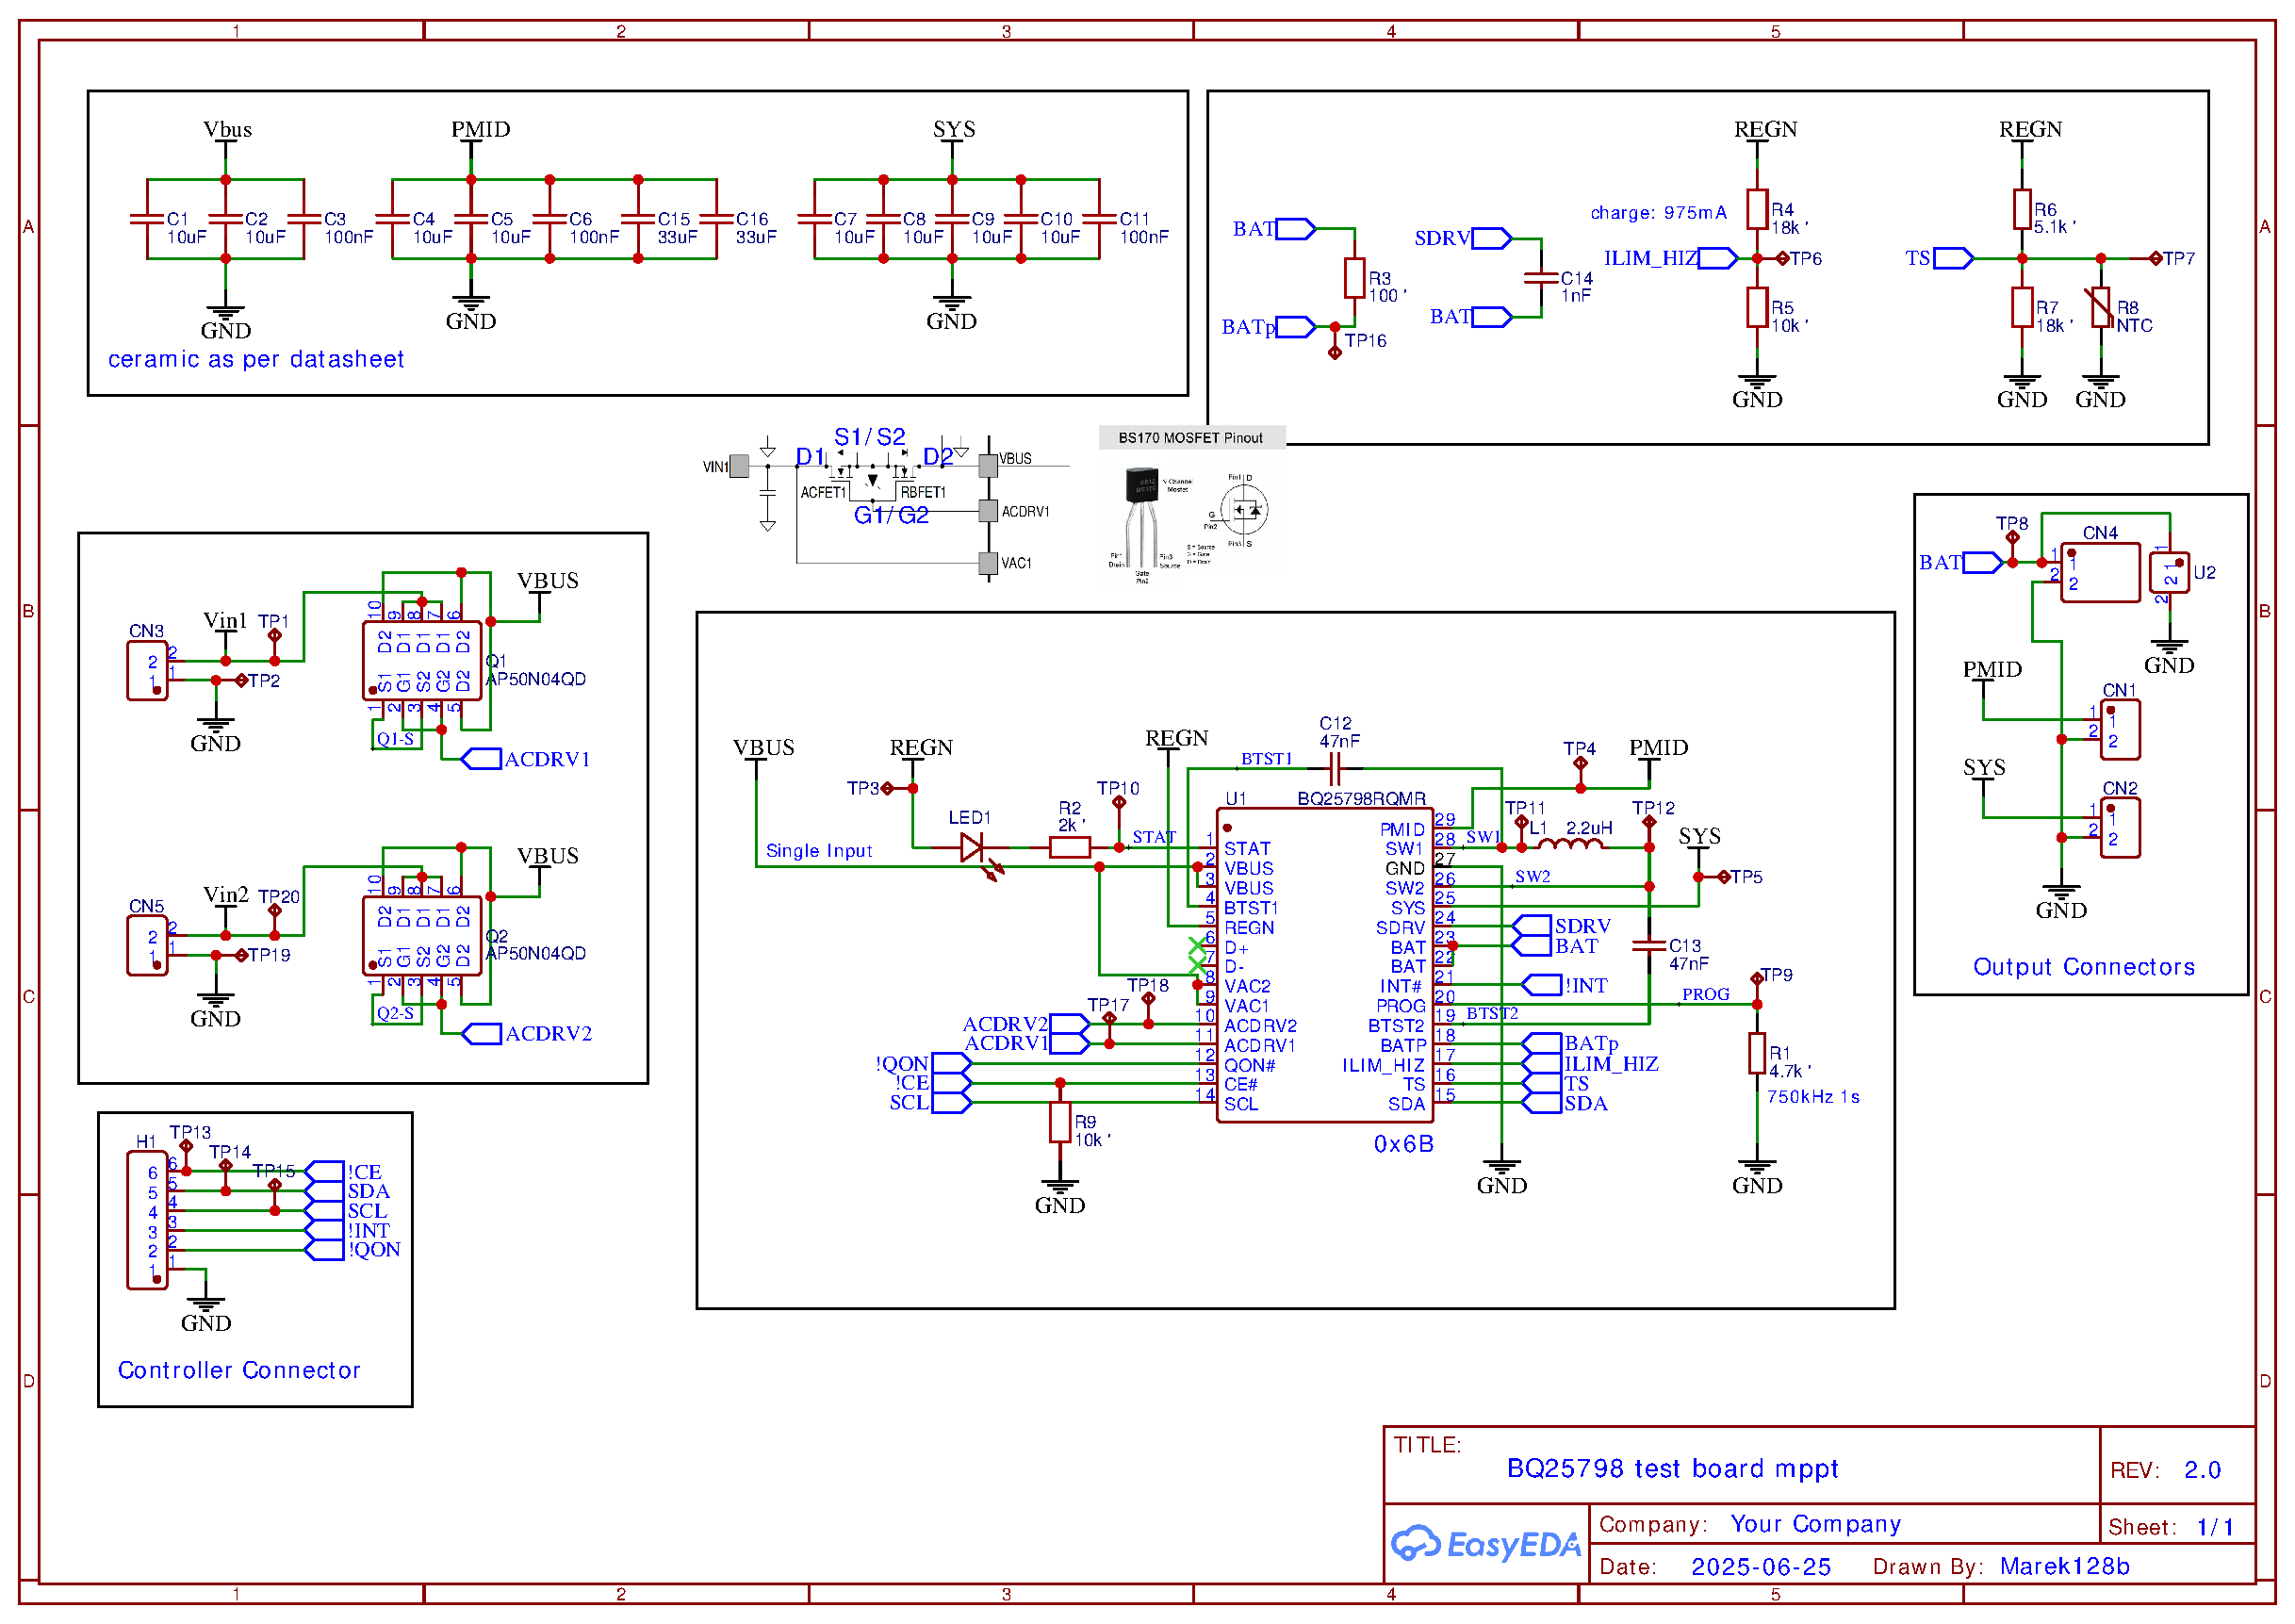
\includegraphics[width=\linewidth]{Schematic_BQ25798-test-board-mppt-solar_2025-10-29.png}
    \caption{Schematics BQ25798 Test Board MPPT Solar}
    \label{img:schematics-V2.0}
\end{figure}

% ##### Changelog V1.0 to V2.0 ############################################################################################
\section{change log}
\subsection{Mistakes V1.0}
\begin{enumerate}
    \item no Marking on PCB of min max Voltages.
    \item CE Pin not having a resistor to pull LOW to enable chip.
    \item too small footprints for soldering. 
\end{enumerate}

\subsection{V2.0 changes}
\begin{enumerate}
    \item Added support for Dual Power Input
    \item Added Backup Mode Support
    \item changed charging current to \(\approx\) 1A
    \item changed Voltage divider for NTC temperature
    \item changed PCB layout to accommodate new 2 inputs and outputs
    \item added better description to PCB
\end{enumerate}

% ##### References ########################################################################################################
\newpage
\nocite{*}
\bibliographystyle{IEEEtran}
\bibliography{references}
\end{document}
